\section{Experimental Results}
\ifCLASSOPTIONonecolumn\begin{figure*}[t]
\centering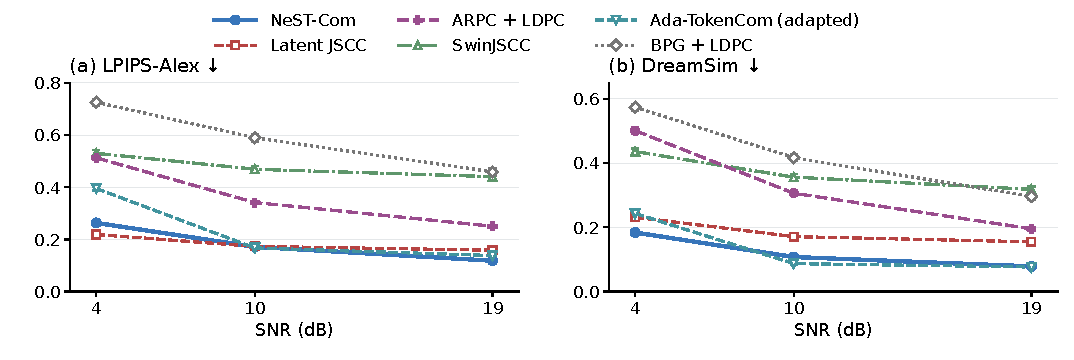
\includegraphics[width=\textwidth]{figure2.pdf}
\caption{Source-referenced perceptual distances on common500 at $N=1024$ and 4/7/10/19~dB. Points and error bars are equal-source means and pointwise 95\% source-bootstrap intervals after averaging three channel outcomes per source. Lower LPIPS-Alex and DreamSim are favorable. Ada denotes the predicted-class, fixed-frame adaptation.}
\label{fig:performance}
\end{figure*}
\fi
\subsection{Experimental Setup}
We use common500 ImageNet validation images~\cite{imagenet}, disjoint cal1000, and Kodak24~\cite{kodak}, with fixed $256\times256$ preprocessing and unchanged ImageNet policies on Kodak. Six systems use $N=1024$; NeST, WHOLE, and Ada also use $N=512$, independently calibrated at 4/10/19~dB. The added 7-dB common500 point uses all six systems at $N=1024$, with policies frozen on 100 calibration images (Supplement~S9).

Our convolutional Latent JSCC maps tokenizer latents to symbols and shares $\Dc$, using MSE, LPIPS, and latent-consistency losses with a 100k-update checkpoint. SwinJSCC~\cite{swinjscc} is trained for 200k updates with RGB MSE and selected by minimum mean calibration MSE. Both use 20\,000 training images and are adapted to $256\times256$ and $N=1024$. Digital baselines include adaptive BPG~\cite{bpg} + LDPC. We implement ARPC~\cite{arpc} with LDPC/QAM and adapt Ada-TokenCom~\cite{adatokencom} to fixed frames, counting captions, classes, and protocol overhead within the symbol budget. Ada retains LlamaGen-L/VQ16 and prefix arithmetic coding, with a fixed ConvNeXt predicting a paid 10-bit class. Its sampled tail uses CFG=4, $T=1$, top-$k=2000$, and top-$p=1$ (Supplement~S1.2).

At both budgets, NeST, WHOLE, and Ada select QPSK rate 2/3, 16-QAM rate 2/3, and 64-QAM rate 5/6 at 4/10/19~dB. In that order, NeST/WHOLE targets are $(7,25)/(7,0)$, $(8,126)/(9,0)$, and $(10,0)/(10,0)$ at $N=1024$; they are $(5,27)/(6,0)$, $(7,0)/(7,0)$, and $(8,84)/(8,0)$ at $N=512$. Ada permits up to 256 tokens before fitting.

The primary reconstruction measures are source-referenced LPIPS-Alex~\cite{lpips} and DreamSim~\cite{dreamsim}. PSNR measures pixel fidelity, and CLIP ViT-L/14 image--image cosine (CLIP-I) measures feature similarity~\cite{clip}. Frozen FP32 preprocessing uses $224\times224$ bicubic-antialias inputs for DreamSim/CLIP. We average three channel outcomes per image, including gray failures, before computing equal-source means and direct source-paired 95\% bootstrap intervals (10\,000 resamples). The endpoint and receiver controls use a fixed 100-image subset.

\ifCLASSOPTIONonecolumn\else\begin{figure*}[t]
\centering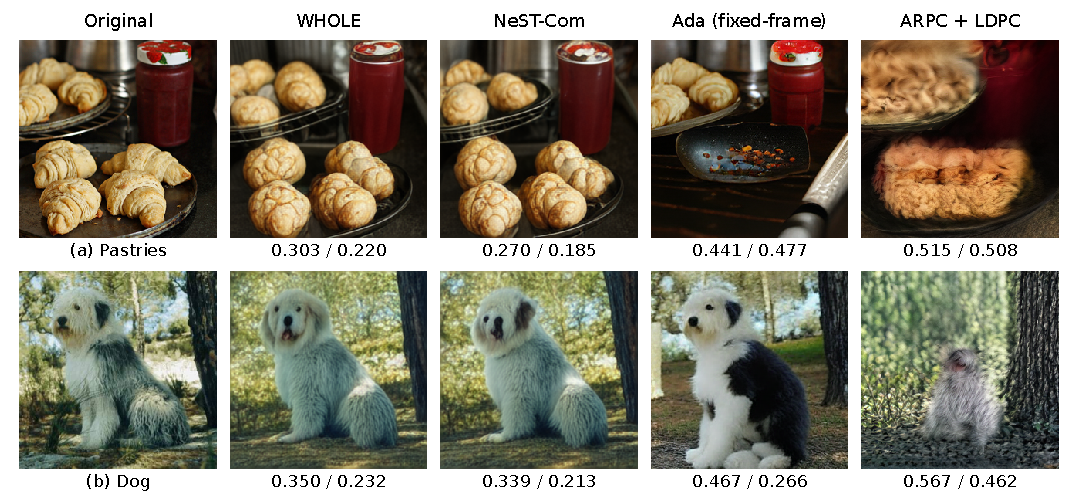
\includegraphics[width=\textwidth]{figure3.pdf}
\caption{Qualitative reconstructions of two fixed development examples at $N=1024$ and 4~dB. Values denote LPIPS-Alex$\downarrow$ / DreamSim$\downarrow$ for each displayed realization. Ada denotes the predicted-class, fixed-frame adaptation.}
\label{fig:qualitative}
\end{figure*}
\fi
\subsection{Effect of Within-Scale Transmission}
\begin{table}[t]
\caption{Within-scale endpoint and receiver evidence. (A) Main common500 policies, PARTIAL minus WHOLE. (B) Fixed 100-source model/MCS/maximum-endpoint control. (C) Ordered interventions on the same 100 sources and actual prefixes. Brackets give source-paired 95\% CIs.}
\label{tab:internal}
\centering\footnotesize
\setlength{\tabcolsep}{2.5pt}
\begin{tabular}{ccc}
\toprule
\multicolumn{3}{l}{(A) Main policies at $N=1024$} \\
SNR & Util. W$\to$P (\%) & $\Delta$LPIPS [95\% CI] \\
\midrule
4 & 73.81 $\to$ 93.08 & $-0.0246\;[-0.0262,-0.0230]$ \\
10 & 77.70 $\to$ 95.21 & $-0.0273\;[-0.0296,-0.0249]$ \\
19 & 85.24 $\to$ 94.73 & $-0.0052\;[-0.0056,-0.0048]$ \\
\midrule
\multicolumn{3}{l}{(B) Fixed-granularity diagnostic, 10 dB} \\
Grid (candidates) & Utilization (\%) & LPIPS \\
Whole (7) & 78.15 & 0.2018 \\
Half (13) & 89.21 & 0.1838 \\
Quarter (25) & 95.38 & 0.1752 \\
Eighth (49) & 97.39 & 0.1729 \\
\midrule
\multicolumn{3}{l}{(C) Receiver interventions: $\Delta$LPIPS [95\% CI]} \\
SNR & B0$-$A0 & C0$-$B0 \\
10 & $-0.0100$ & $-0.0166$ \\
 & $[-0.0120,-0.0080]$ & $[-0.0205,-0.0129]$ \\
19 & $-0.0051$ & $+0.0000$ \\
 & $[-0.0060,-0.0043]$ & $[0.0000,0.0000]$ \\
\bottomrule
\end{tabular}
\par\smallskip\parbox{\columnwidth}{\footnotesize Boundary tokens: A0, unused; B0, residual correction only; C0, residual correction and conditioning update. All three use the received complete coarse scales.}
\end{table}

Table~\ref{tab:internal}(A) compares WHOLE and NeST-Com (PARTIAL) with a shared tokenizer, prior, entropy coder, and $\Dc$. Their separately calibrated policies select the same MCS at each SNR. At $N=1024$, 10~dB, within-scale transmission increases source-bit utilization from 77.70\% to 95.21\%. Mean LPIPS decreases from 0.198718 to 0.171465, and DreamSim from 0.131728 to 0.107680, corresponding to relative metric reductions of 13.7\% and 18.3\%. The paired DreamSim difference is $-0.0240\,[-0.0270,-0.0212]$. Both distances improve at all three SNRs, with PSNR gains of 0.32--0.70~dB (Supplement~S2.4). Kodak also has lower LPIPS at all three SNRs under the unchanged ImageNet policies (S2.5).

Block~B fixes the 100 sources, model, MCS, maximum endpoint, and fitting rule. Whole-to-Eighth refinement raises utilization from 78.15\% to 97.39\% and lowers LPIPS from 0.201821 to 0.172939. Compared with the predefined Quarter grid, Eighth reduces LPIPS by $0.00223\,[0.00131,0.00323]$ and increases PSNR by $0.123\,[0.079,0.169]$~dB. Its DreamSim difference is $-0.00073\,[-0.00196,0.00048]$. Both grids use ten prior-scale calls and one 680-token coding traversal, with 25/49 independent finalizations, respectively (Supplement~S5.1).

Block~C holds actual received prefixes fixed. At 10~dB, residual correction (B0--A0) reduces LPIPS by 0.01003; subsequent conditioning update (C0--B0) reduces it by 0.01662. Corresponding DreamSim differences are $-0.00845\,[-0.01136,-0.00564]$ and $-0.01537\,[-0.01988,-0.01111]$. At 19~dB the boundary lies in the final scale, so the conditioning update has zero effect.

With the 10-dB WHOLE/PARTIAL policies frozen, both methods reject all 300 receptions at an actual SNR of 8~dB and none at 10/12~dB. Their recovered prefixes and per-source reconstructions coincide between 10 and 12~dB, preserving the within-scale gain after successful delivery (Supplement~S5).

\subsection{Comparison With Existing Methods}
\ifCLASSOPTIONonecolumn\begin{figure*}[t]
\centering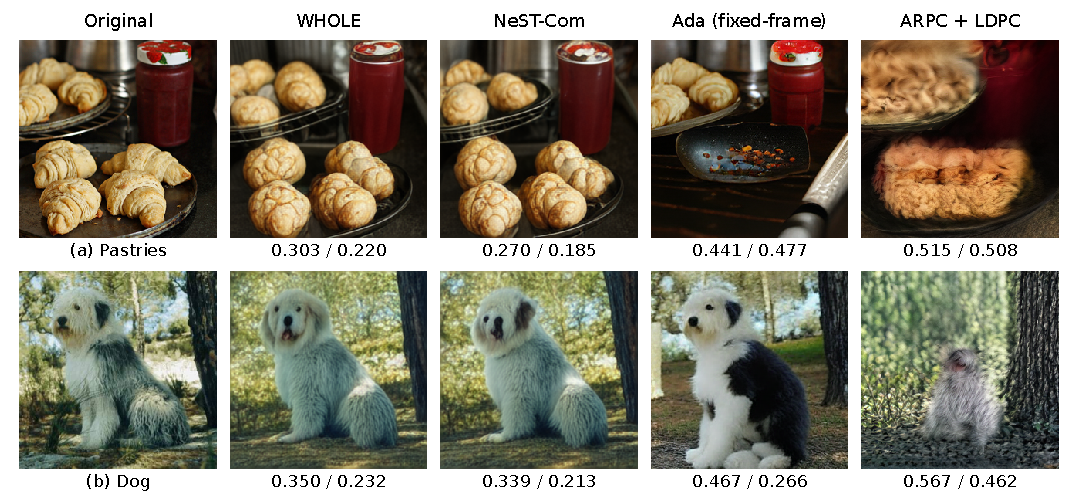
\includegraphics[width=\textwidth]{figure3.pdf}
\caption{Qualitative reconstructions of two fixed development examples at $N=1024$ and 4~dB. Values denote LPIPS-Alex$\downarrow$ / DreamSim$\downarrow$ for each displayed realization. Ada denotes the predicted-class, fixed-frame adaptation.}
\label{fig:qualitative}
\end{figure*}
\fi
\begin{table}[t]
\caption{Pixel fidelity and image-feature similarity on common500 at $N=1024$. Each cell is PSNR (dB)$\uparrow$ / CLIP-I$\uparrow$. Ada denotes the fixed-frame adaptation. Values are source means.}
\label{tab:external}
\centering\footnotesize
\setlength{\tabcolsep}{3pt}
\begin{tabular}{lccc}
\toprule Method & 4 dB & 10 dB & 19 dB \\
\midrule
NeST-Com & 17.448 / 0.821 & 20.014 / 0.873 & 22.164 / 0.900 \\
Latent JSCC & 19.658 / 0.741 & 20.803 / 0.789 & 21.245 / 0.804 \\
SwinJSCC & 21.671 / 0.627 & 23.026 / 0.669 & 23.698 / 0.697 \\
BPG + LDPC & 20.743 / 0.586 & 22.543 / 0.635 & 24.230 / 0.684 \\
ARPC + LDPC & 14.184 / 0.644 & 16.471 / 0.713 & 18.199 / 0.788 \\
Ada (adapted) & 13.332 / 0.828 & 19.559 / 0.884 & 20.938 / 0.892 \\
\bottomrule
\end{tabular}
\end{table}

Fig.~\ref{fig:performance} compares six systems at $N=1024$. NeST has lower LPIPS and DreamSim than SwinJSCC, BPG, and ARPC throughout. SwinJSCC and BPG have higher PSNR at 4/10/19~dB (Table~\ref{tab:external}). Against Latent JSCC, NeST has lower DreamSim at all four points; Latent JSCC has lower LPIPS and higher PSNR at 4/7~dB.

At 4~dB, NeST's LPIPS/DreamSim are 0.263/0.184 versus Ada's 0.395/0.243. At 7~dB, NeST lowers LPIPS by $0.0584\,[0.0533,0.0637]$ versus Ada; their DreamSim difference is $0.0012\,[-0.0052,0.0074]$, with no clear advantage. Ada has lower LPIPS/DreamSim at 10~dB and higher CLIP-I at 4/10~dB. At 19~dB NeST has lower LPIPS, but Ada has slightly lower DreamSim. NeST has higher PSNR than Ada throughout. NeST/WHOLE/Ada have no failures in 1500 trials per original SNR (Supplement~S2). At 7~dB, NeST/Ada/BPG reject 6/7/11 of 1500 receptions each; gray failures remain in the means (S9).

On the fixed 100-source control set, replacing Ada's sampled tail with argmax increases both LPIPS and DreamSim at $N=512$, 4/10~dB and $N=1024$, 10~dB; all six paired intervals exclude zero (Supplement~S3). Thus sampling gives the stronger perceptual baseline at these tested points.

Fig.~\ref{fig:qualitative} shows fixed 4-dB development cases. WHOLE and NeST retain scene layout but round off croissant shapes. NeST better preserves the dog's dark ear; Ada changes plate contents and coat pattern, while ARPC changes shapes and pose. Supplement~S8 retains all methods and the 10-dB view.

NeST's mean TX/RX times at $N=1024$, 10~dB are 220.89/398.82~ms (RTX PRO 6000, six cores, batch one, 16 sources, three repetitions; Supplement~S5). ARPC's 100-source payload audit, including paid caption fields, is in S1.3.

\subsection{Transmission With a Reduced Symbol Budget}
\begin{table}[t]
\caption{Reduced-budget perceptual differences on common500 at $N=512$. (A) NeST-Com minus WHOLE with shared models. (B) NeST-Com minus the fixed-frame Ada-TokenCom adaptation. Brackets give direct source-paired 95\% CIs; negative values favor NeST-Com.}
\label{tab:reduced}
\centering\footnotesize
\setlength{\tabcolsep}{4pt}
\begin{tabular}{ccc}
\toprule SNR & $\Delta$LPIPS & $\Delta$DreamSim \\
\midrule
\multicolumn{3}{l}{(A) NeST-Com minus WHOLE} \\
4 & $-0.0299$ & $-0.0428$ \\
 & $[-0.0337,-0.0264]$ & $[-0.0483,-0.0373]$ \\
10 & $-0.0155$ & $-0.0127$ \\
 & $[-0.0170,-0.0137]$ & $[-0.0150,-0.0104]$ \\
19 & $-0.0275$ & $-0.0241$ \\
 & $[-0.0288,-0.0262]$ & $[-0.0264,-0.0220]$ \\
\midrule
\multicolumn{3}{l}{(B) NeST-Com minus Ada (adapted)} \\
4 & $-0.1890$ & $-0.1029$ \\
 & $[-0.1966,-0.1814]$ & $[-0.1142,-0.0917]$ \\
10 & $-0.1384$ & $-0.0660$ \\
 & $[-0.1440,-0.1328]$ & $[-0.0747,-0.0573]$ \\
19 & $-0.0245$ & $+0.0139$ \\
 & $[-0.0280,-0.0212]$ & $[0.0103,0.0173]$ \\
\bottomrule
\end{tabular}
\par\smallskip\begin{minipage}{\columnwidth}\footnotesize
Successful receptions (4/10/19~dB), each out of 1500: NeST 1496/1499/1500; WHOLE 1493/1500/1500; Ada 1495/1500/1500. All failures are body-CRC rejections retained as gray.
\end{minipage}
\end{table}

Table~\ref{tab:reduced}(A) tests within-scale transmission at $N=512$. NeST improves LPIPS and DreamSim over WHOLE at all three SNRs, with all paired intervals excluding zero. PSNR improves by 0.39--0.79~dB and CLIP-I also increases. At 10~dB both methods select target $(7,0)$ and 16-QAM rate 2/3. Both fall back from this target for 99.6\% of sources, but NeST retains a within-scale prefix for 89.0\%. Mean retained tokens increase from 91.3 to 107.9, raising source-bit utilization from 79.30\% to 93.46\%.

Table~\ref{tab:reduced}(B) gives the complete-system comparison with Ada. NeST has lower LPIPS throughout and lower DreamSim at 4/10~dB; Ada has lower DreamSim at 19~dB and higher CLIP-I throughout. WHOLE itself has lower mean LPIPS and DreamSim than Ada at 4/10~dB, and within-scale transmission adds the gains in block~A. NeST exceeds Ada in PSNR by 1.74--4.18~dB. Joint-success comparisons retain all 500 sources and the same LPIPS/DreamSim directions (Supplement~S2.3); S4 examines completion versus coarse-only decoding.
